\documentclass[letter,11pt]{article}

\usepackage[spanish,es-nodecimaldot]{babel}
\usepackage[utf8]{inputenc}

\usepackage{lmodern}
\usepackage[T1]{fontenc}
\usepackage{textcomp}

\usepackage{framed}
\usepackage[svgnames]{xcolor}
\colorlet{shadecolor}{Gainsboro!50}

\usepackage[labelfont=bf]{caption}
\usepackage{graphicx}
\usepackage{pstricks}

\usepackage{anysize}
\marginsize{3cm}{2cm}{2cm}{3cm}

\usepackage{siunitx}
\usepackage{amsmath}
\usepackage{array}
\usepackage{alltt}

\usepackage{caption}
\newcommand{\source}[1]{\vspace{-11pt} \caption*{\small{\textbf{Nota:} {#1}}}}

\usepackage{fancyhdr}
\usepackage{lastpage}
\pagestyle{fancy}
\fancyhf{}
\fancyhead[LE,RO]{Laboratorio de Física Básica II}
\fancyfoot[CO,CE]{\thepage\ de \pageref{LastPage}}

\special{papersize=215.9mm,279.4mm}

\usepackage[
    pdfauthor={Carlos Eduardo Caballero Burgoa},%
    pdftitle={Laboratorio de Física Básica II},%
    pdfsubject={Péndulo físico},%
    colorlinks,%
    citecolor=black,%
    filecolor=black,%
    linkcolor=black,%
    urlcolor=black,
    breaklinks]{hyperref}
\usepackage{breakurl}

\newcommand{\blankpage}{
\newpage
\thispagestyle{empty}
\mbox{}
\newpage
}

\renewcommand{\arraystretch}{1.2}

\title{Informe 4: Péndulo físico}
\author{Carlos Eduardo Caballero Burgoa \\
    \small{\href{mailto:200201226@est.umss.edu}{200201226@est.umss.edu}}
}
\date{12 de mayo de 2021}

\begin{document}

\maketitle
\begin{center}
    \textbf{Grupo}: J2 (Miércoles)\\
    \textbf{Docente}: Ing. Milka Mónica Torrico Troche\\
    \textbf{Carrera}: Ing. Electromecánica
\end{center}

\begin{abstract}
Este documento detalla el experimento realizado para calcular el valor del radio
de giro ($k$) de un péndulo físico respecto a su centro de masa, además del
valor de la gravedad local ($g$); para esto se realizó primeramente el calculo
del centro de masa sobre el objeto experimental, luego se realizó dos mediciones
de la oscilaciones del objeto dada una distancia determinada al centro de masa;
y posteriormente se calculó la relación funcional entre el periodo ($T$) y la
distancia entre el eje de oscilación y el centro de masa ($b$) después de
linealizar la curva y ajustarla con el método de mínimos cuadrados, finalmente
se determinaron los valores deseados, resultando ser:
$(0.1501 \pm 0.0000014) [m]; 0.0009\%$ para el radio de giro, y
$(9.78 \pm 0.08) [m/s^2]; 0.77\%$ para la gravedad.
\end{abstract}

\section{Introducción}

Un péndulo físico es cualquier péndulo real que usa un cuerpo de tamaña finito,
en contraste con el modelo idealizado de péndulo simple en el que toda la masa
se concentra en un punto.

\begin{figure}
\centering
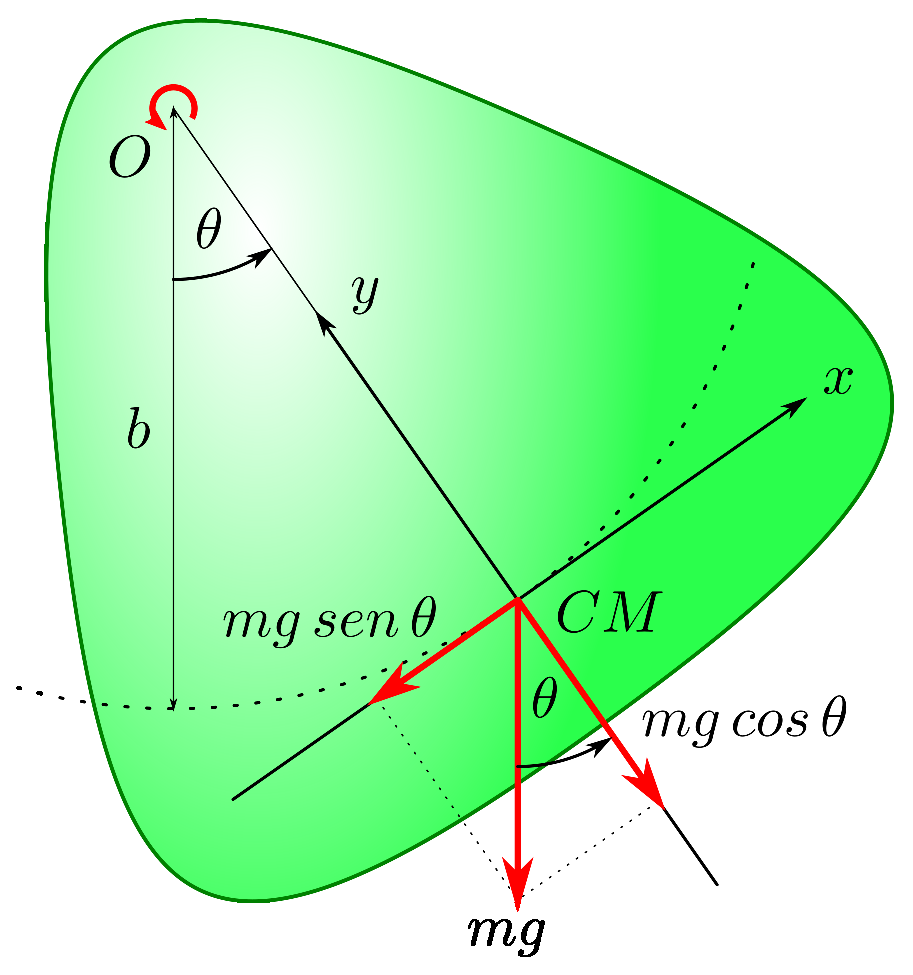
\includegraphics[width=0.34\textwidth]{resources/f1.eps}
\caption{Dinámica de un péndulo físico.}
\label{figura1}
\source{Física Universitaria Volumen I (p. 455), \\
Young, Hugh D. y Freedman, Roger A., 2013, Pearson.}
\end{figure}

En la \textbf{Figura \ref{figura1}} se detallan las fuerzas que actúan sobre el
cuerpo rígido que puede girar sin fricción alrededor de un eje que pasa por el
punto $O$.

En la posición de equilibrio, el centro de masa $CM$ y el eje de oscilación $O$
se encuentran sobre la misma linea vertical. mientras el cuerpo rígido oscile
alrededor del equilibrio este formará un ángulo $\theta$ con la vertical. La
distancia entre $O$ y el centro de masa del cuerpo rígido $CM$ es $b$, y el
momento de inercia del cuerpo rígido alrededor del eje de rotación a través de
$O$ es $I$ y la masa total es $m$ \cite{Young&Freedman}.

Cuando el cuerpo rígido se desplaza, el peso $mg$ causa un torque de
restitución:

\begin{equation}
    \tau = -(mg)\,(b\, sen(\theta))
\label{torque}
\end{equation}
\vspace{0.10cm}

De la segunda ley de \emph{Newton} para el movimiento rotatorio, se sabe que:

\begin{equation}
    \tau = I \alpha
\label{segundaley}
\end{equation}
\vspace{0.10cm}

Donde $\alpha$ es la aceleración angular, la cual es la segunda derivada del
desplazamiento angular:

\begin{equation}
    \alpha = \frac{d^2\theta}{dt^2}
\label{segundaderivada}
\end{equation}
\vspace{0.10cm}

Reemplazando $\tau$ de la \textbf{Ecuación \ref{torque}} y $\alpha$  de la
\textbf{Ecuación \ref{segundaderivada}}, en la
\textbf{Ecuación \ref{segundaley}}, se obtiene:

\begin{equation*}
    -(mg)\,(b\, sen(\theta)) = I \frac{d^2\theta}{dt^2}
\end{equation*}
\begin{equation}
    \frac{d^2\theta}{dt^2} = - \frac{mgb}{I}\, sen(\theta)
\label{diferencial}
\end{equation}
\vspace{0.10cm}

Si se consideran tan solo oscilaciones de pequeña amplitud, de modo que el
ángulo $\theta$ sea siempre suficientemente pequeño, entonces el valor del
$sen\, (\theta)$ será muy próximo al valor de $\theta$ expresado en radianes
($sen\, (\theta) \cong \theta$, para $\theta$ suficientemente pequeño), como
se aprecia en el \textbf{Cuadro \ref{cuadro1}} \cite{WIKI1}.

\begin{table}[!h]
\begin{center}
\begin{tabular}{|>{\centering}m{0.50cm}<{\centering}
                |>{\centering}m{1.25cm}<{\centering}
                |>{\centering}m{1.25cm}<{\centering}
                |>{\centering}m{2.50cm}<{\centering}|
                |>{\centering}m{0.50cm}<{\centering}
                |>{\centering}m{1.25cm}<{\centering}
                |>{\centering}m{1.25cm}<{\centering}
                |>{\centering}m{2.50cm}<{\centering}|}
\hline
$\theta [^\circ]$ & $\theta [rad]$ & $sen\, (\theta)$ & diferencia (\%) &
$\theta [^\circ]$ & $\theta [rad]$ & $sen\, (\theta)$ & diferencia (\%)
    \tabularnewline \hline
\hline
 0 & 0.00000 & 0.00000 & 0.00 & 15 & 0.26180 & 0.25882 & 1.15
    \tabularnewline \hline
 2 & 0.03491 & 0.03490 & 0.02 & 20 & 0.34907 & 0.34202 & 2.06
    \tabularnewline \hline
 5 & 0.08727 & 0.08716 & 0.13 & 25 & 0.43633 & 0.42262 & 3.25
    \tabularnewline \hline
10 & 0.17453 & 0.17365 & 0.51 & 30 & 0.52360 & 0.50000 & 4.72
    \tabularnewline \hline
\end{tabular}
\caption{Comparación entre el valor del ángulo y su función seno.}
\label{cuadro1}
\source{Adaptado de péndulo simple (Wikipedia).}
\end{center}
\end{table}

La \textbf{Ecuación \ref{diferencial}} se reduce a:

\begin{equation}
    \frac{d^2\theta}{dt^2} = - \frac{mgb}{I}\, \theta
\label{oscilador}
\end{equation}
\vspace{0.10cm}

La \textbf{Ecuación \ref{oscilador}} corresponde a un \textbf{oscilador armónico
simple} cuya solución general es:

\begin{equation*}
    \theta(t) = A\, cos\, (\omega\, t + \phi)
\end{equation*}
\vspace{0.10cm}

Donde $A$ representa el máximo desplazamiento angular de $\theta$, $\omega$ es
la frecuencia angular, y $\phi$ el desfase. Tanto la magnitud $A$, como $\phi$
son dos constantes determinadas por las condiciones iniciales.

La frecuencia angular ($\omega$) esta determinada por:

\begin{equation*}
    \omega = \sqrt{\frac{mgb}{I}}
\end{equation*}
\vspace{0.10cm}

Considerando que $\omega = 2\pi / T$, el periodo de oscilación para el péndulo
físico es:

\begin{equation}
    T = 2\pi\, \sqrt{\frac{I}{mgb}}
\label{periodo}
\end{equation}
\vspace{0.10cm}

El \textbf{radio de giro} ($k$) se define como la distancia desde el eje de giro
a un punto donde podríamos suponer concentrada toda la masa del cuerpo de modo
que el momento de inercia respecto a dicho eje se obtenga como el producto de la
masa del cuerpo por el cuadrado del radio de giro \cite{RADIO}.

Por tanto, es posible definir el momento de inercia en el centro de masa como:

\begin{equation}
    I_{cm} = m k^2
\label{radiodegiro}
\end{equation}
\vspace{0.10cm}

Entonces es posible definir el momento de inercia en el eje de oscilación en
función del radio de giro y la distancia $b$, con la ayuda del teorema de los
ejes paralelos, o teorema de \emph{Steiner}:

\begin{equation}
    I = I_{cm} + mb^2 = m k^2 + m b^2
\label{steiner}
\end{equation}
\vspace{0.10cm}

Reemplazando $I$ de la \textbf{Ecuación \ref{steiner}} en la
\textbf{Ecuación \ref{periodo}}:

\begin{equation}
    T = 2\pi\, \sqrt{\frac{m k^2 + m b^2}{mgb}}
      = 2\pi\, \sqrt{\frac{k^2 + b^2}{gb}}
\label{periodo2}
\end{equation}
\vspace{0.10cm}

Despejando $b^2$ de la \textbf{Ecuación \ref{periodo2}}, se obtiene \cite{GUIA}:

\begin{equation*}
    T^2 = 4\pi^2\, \frac{k^2 + b^2}{gb}
\end{equation*}
\begin{equation*}
    \frac{g}{4\pi^2}\, bT^2 = k^2 + b^2
\end{equation*}
\begin{equation}
    b^2 = -k^2 + \frac{g}{4\pi^2}\, bT^2
\label{funcional}
\end{equation}
\vspace{0.10cm}

Para el experimento se verificará la \textbf{Ecuación \ref{funcional}}. A partir
de una distancia del centro de masa al eje de oscilación ($b$) determinada, se
medirá el tiempo de oscilación del péndulo físico para hallar el periodo ($T$).
Finalmente se determinará el valor del radio de giro ($k$) y la gravedad ($g$)
despejándola de la misma ecuación.

\section{Método experimental}

\begin{figure}
\centering
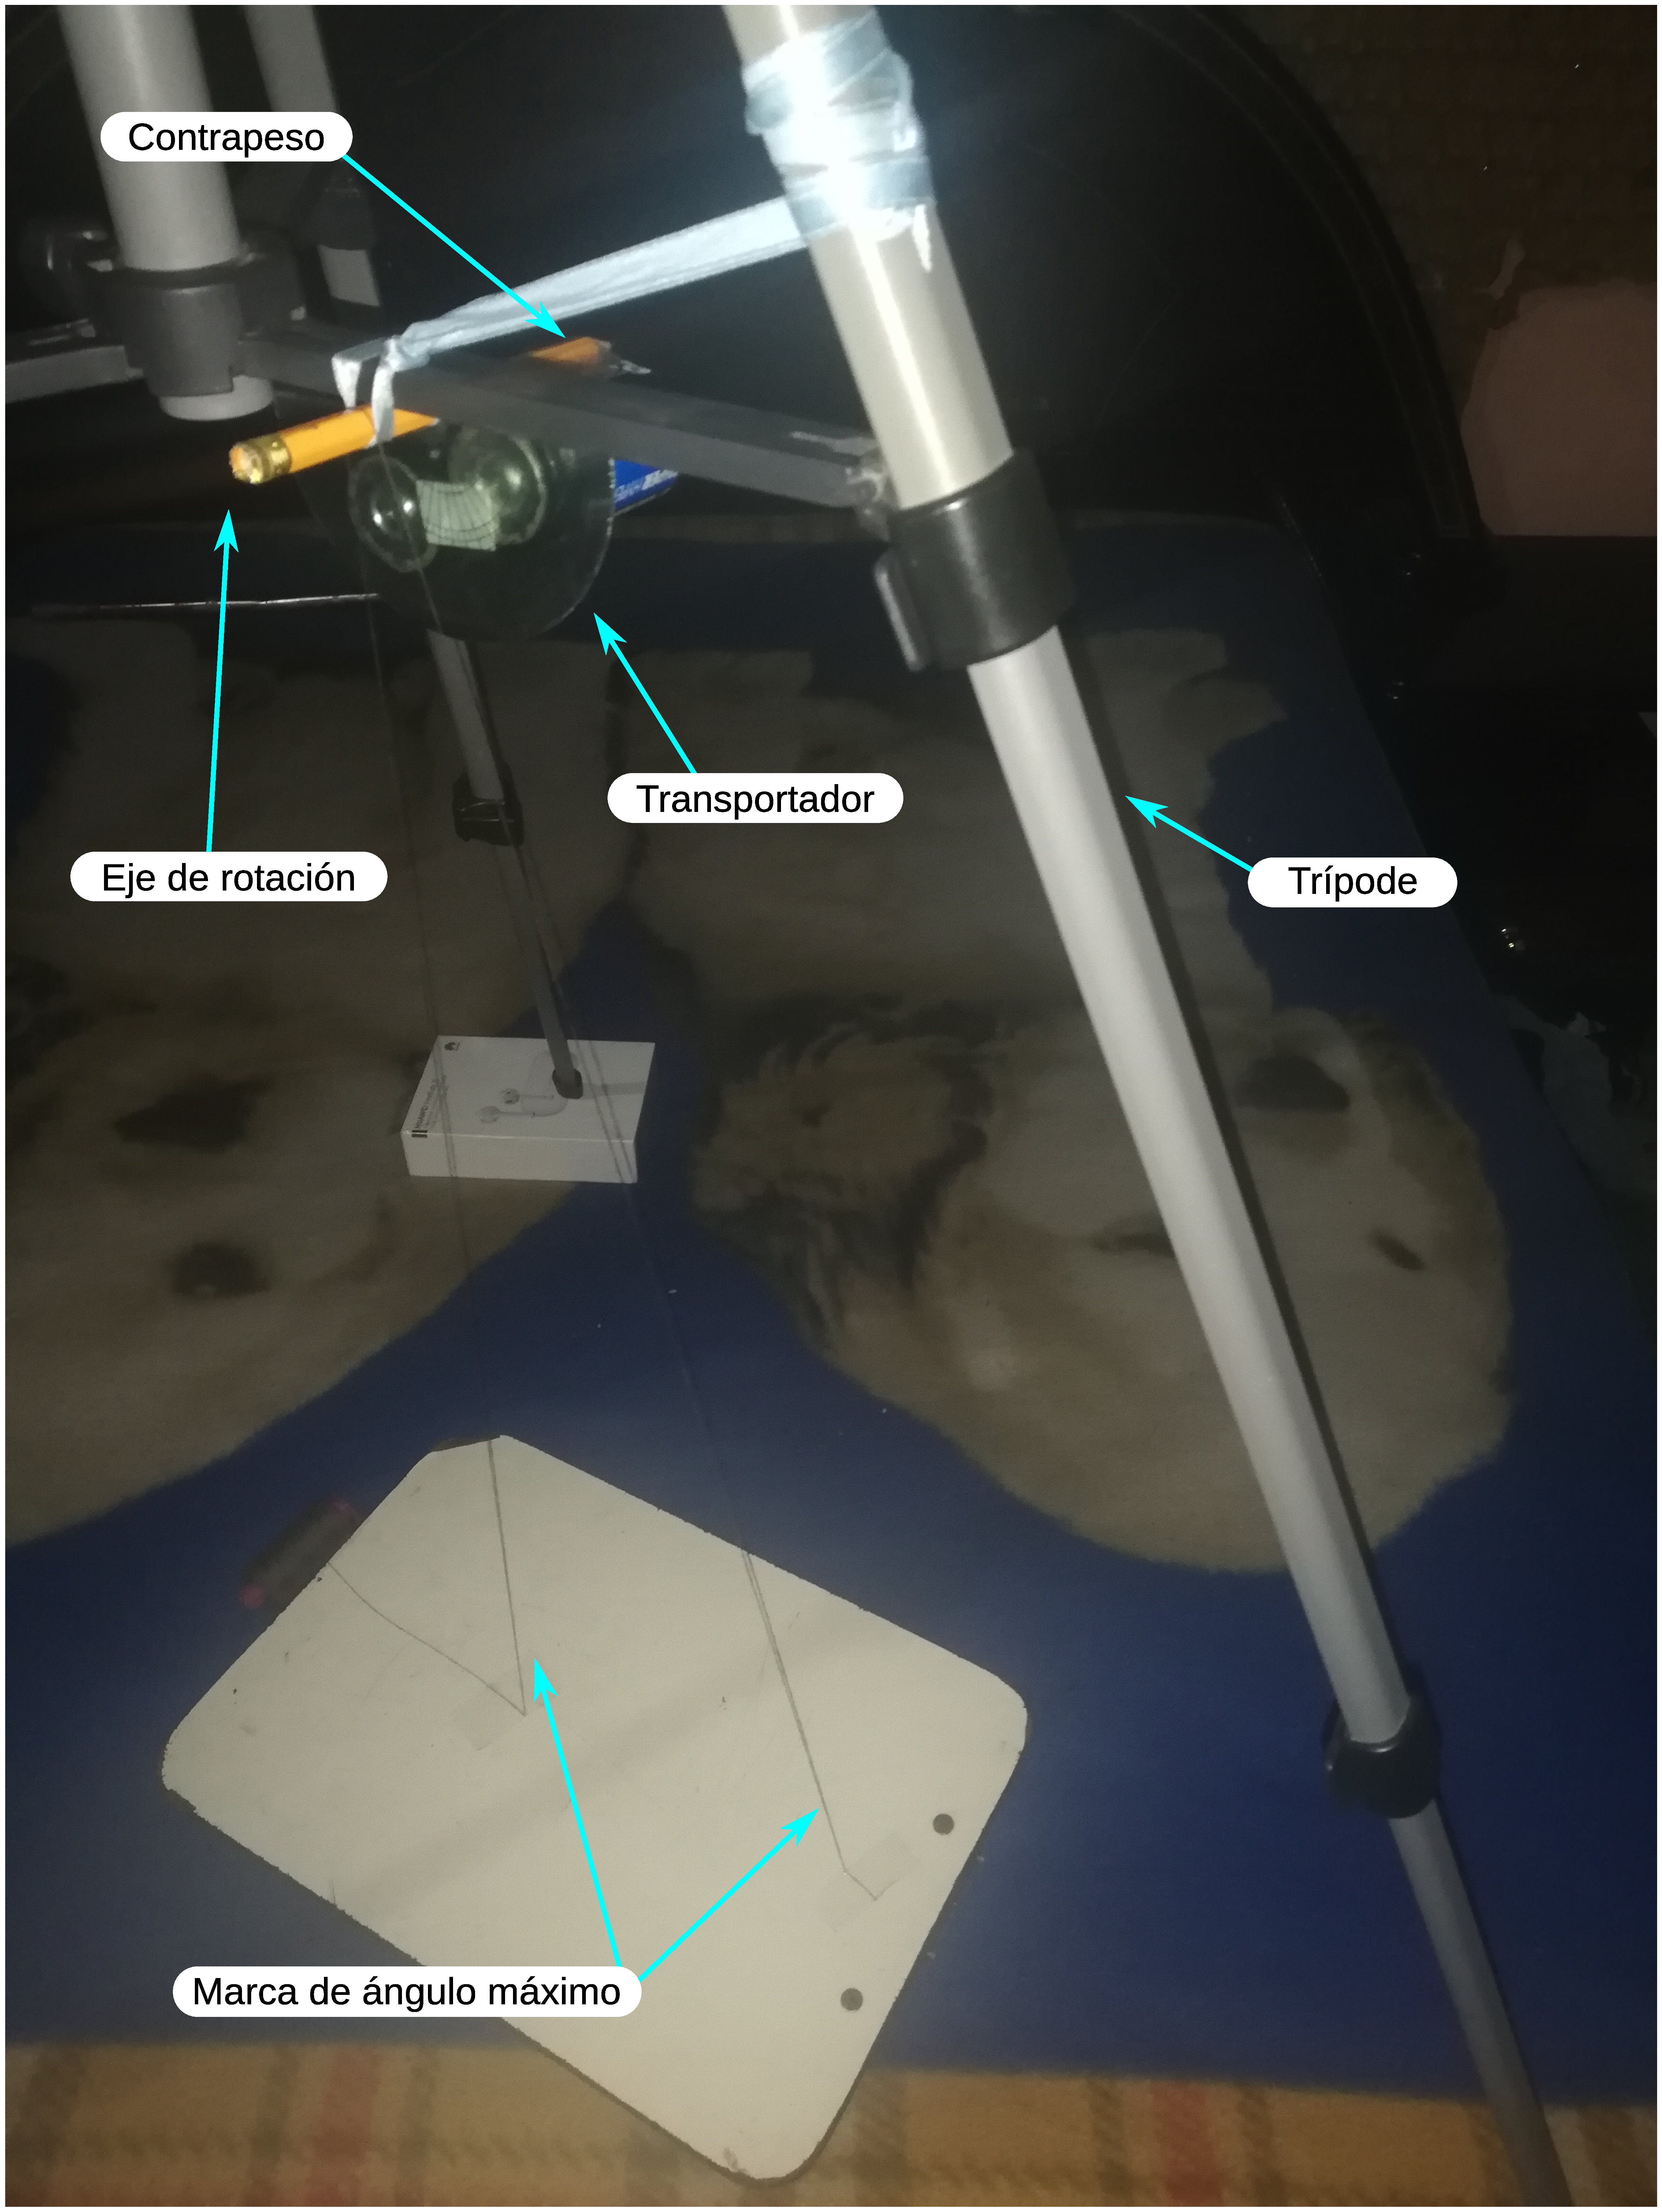
\includegraphics[width=0.70\textwidth]{resources/f2.eps}
\caption{Montaje para el experimento.}
\label{figura2}
\source{Fotografía propia.}
\end{figure}

Para facilitar la medición, se ha armado el equipo mostrado en la
\textbf{Figura \ref{figura2}}, el cual consta de un \textbf{trípode},
previamente nivelado, y un eje de rotación fijado a un contrapeso. Al trípode se
ha sujetado un transportador para marcar con hilo la variación del ángulo, de
forma que la oscilación no exceda los $10^\circ$.

\begin{figure}
\centering
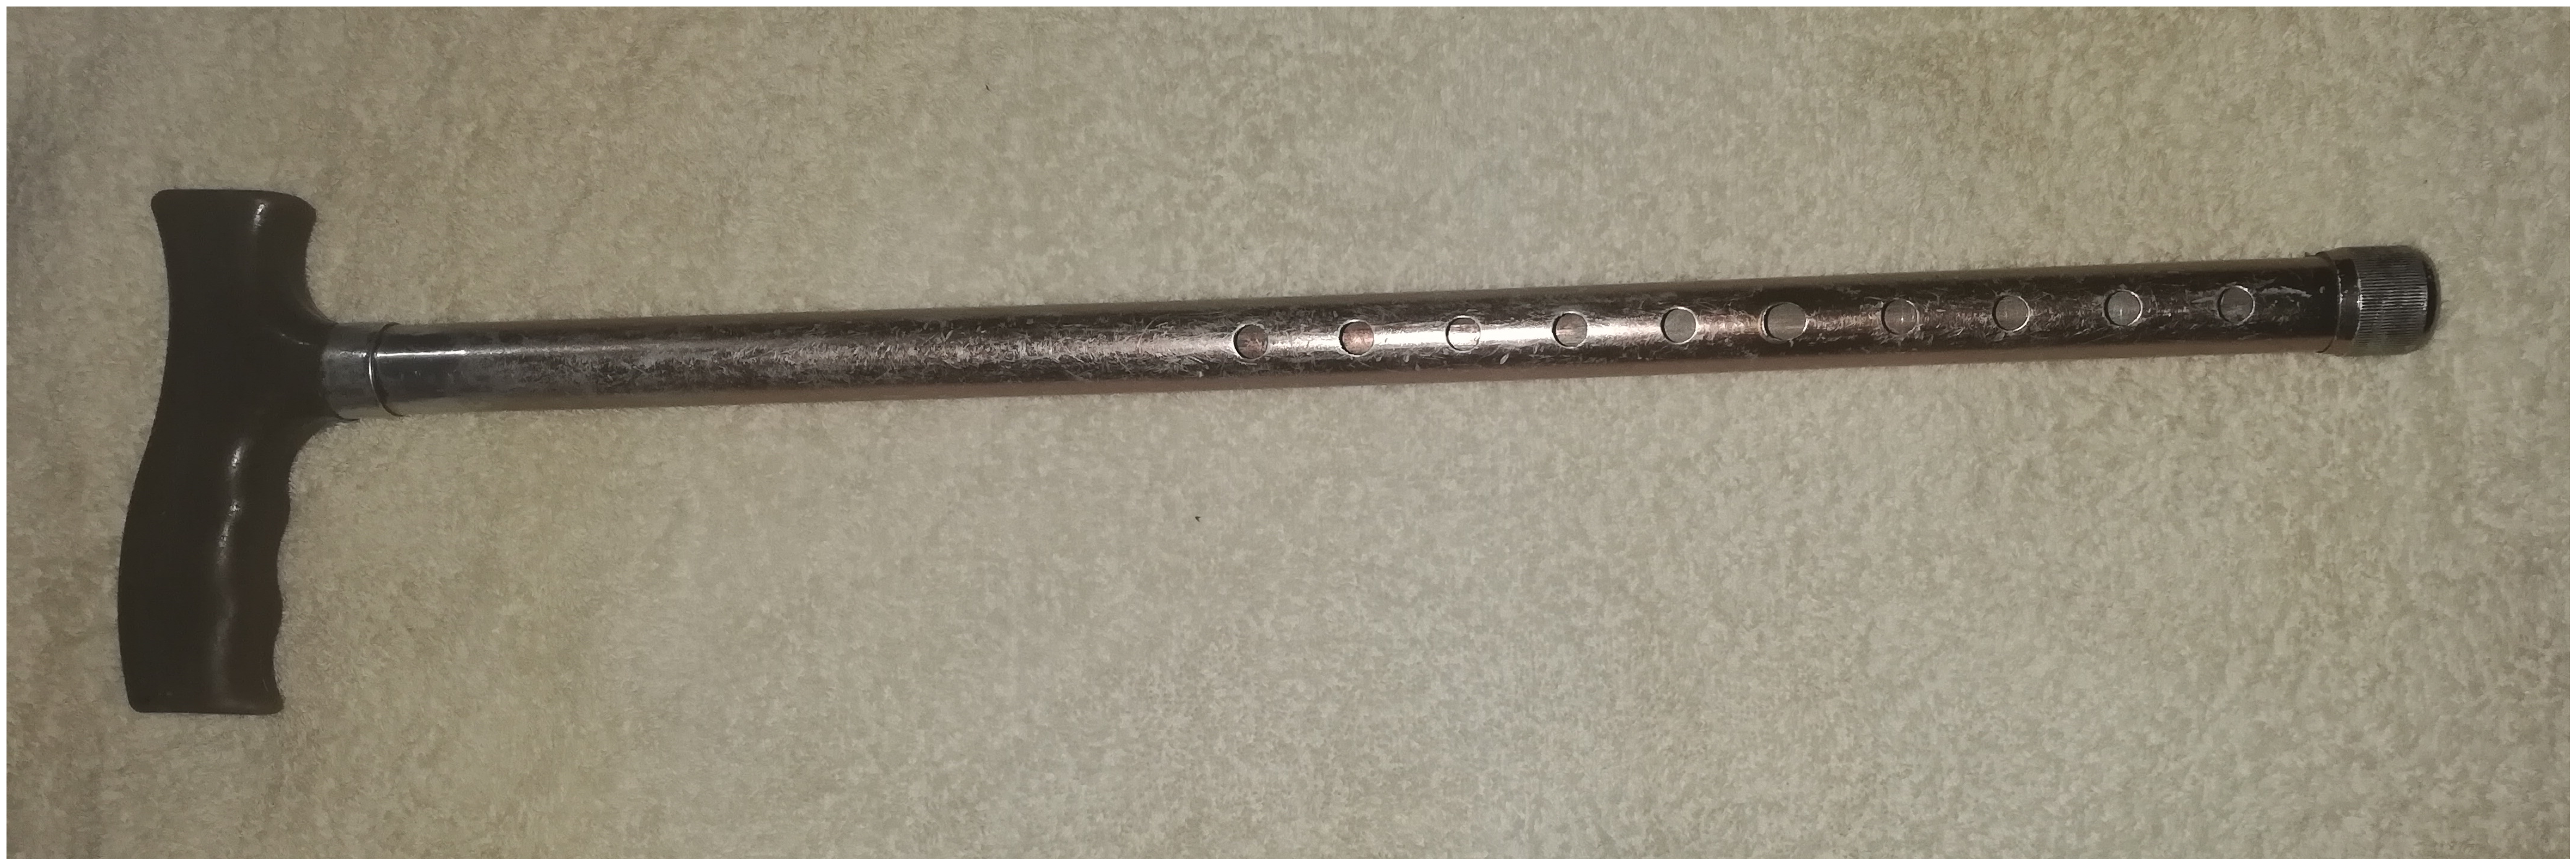
\includegraphics[width=0.65\textwidth]{resources/f3.eps}
\caption{Cuerpo rígido a oscilar.}
\label{figura3}
\source{Fotografía propia.}
\end{figure}

Una vez montado el soporte, se escogió el cuerpo rígido que se haría oscilar, el
cual es un bastón de aluminio cuyo peso es $173.6 [g]$, y que cuenta con varios
orificios del cual puede suspenderse el objeto, como puede apreciarse en la
\textbf{Figura \ref{figura3}}.

\begin{figure}
\centering
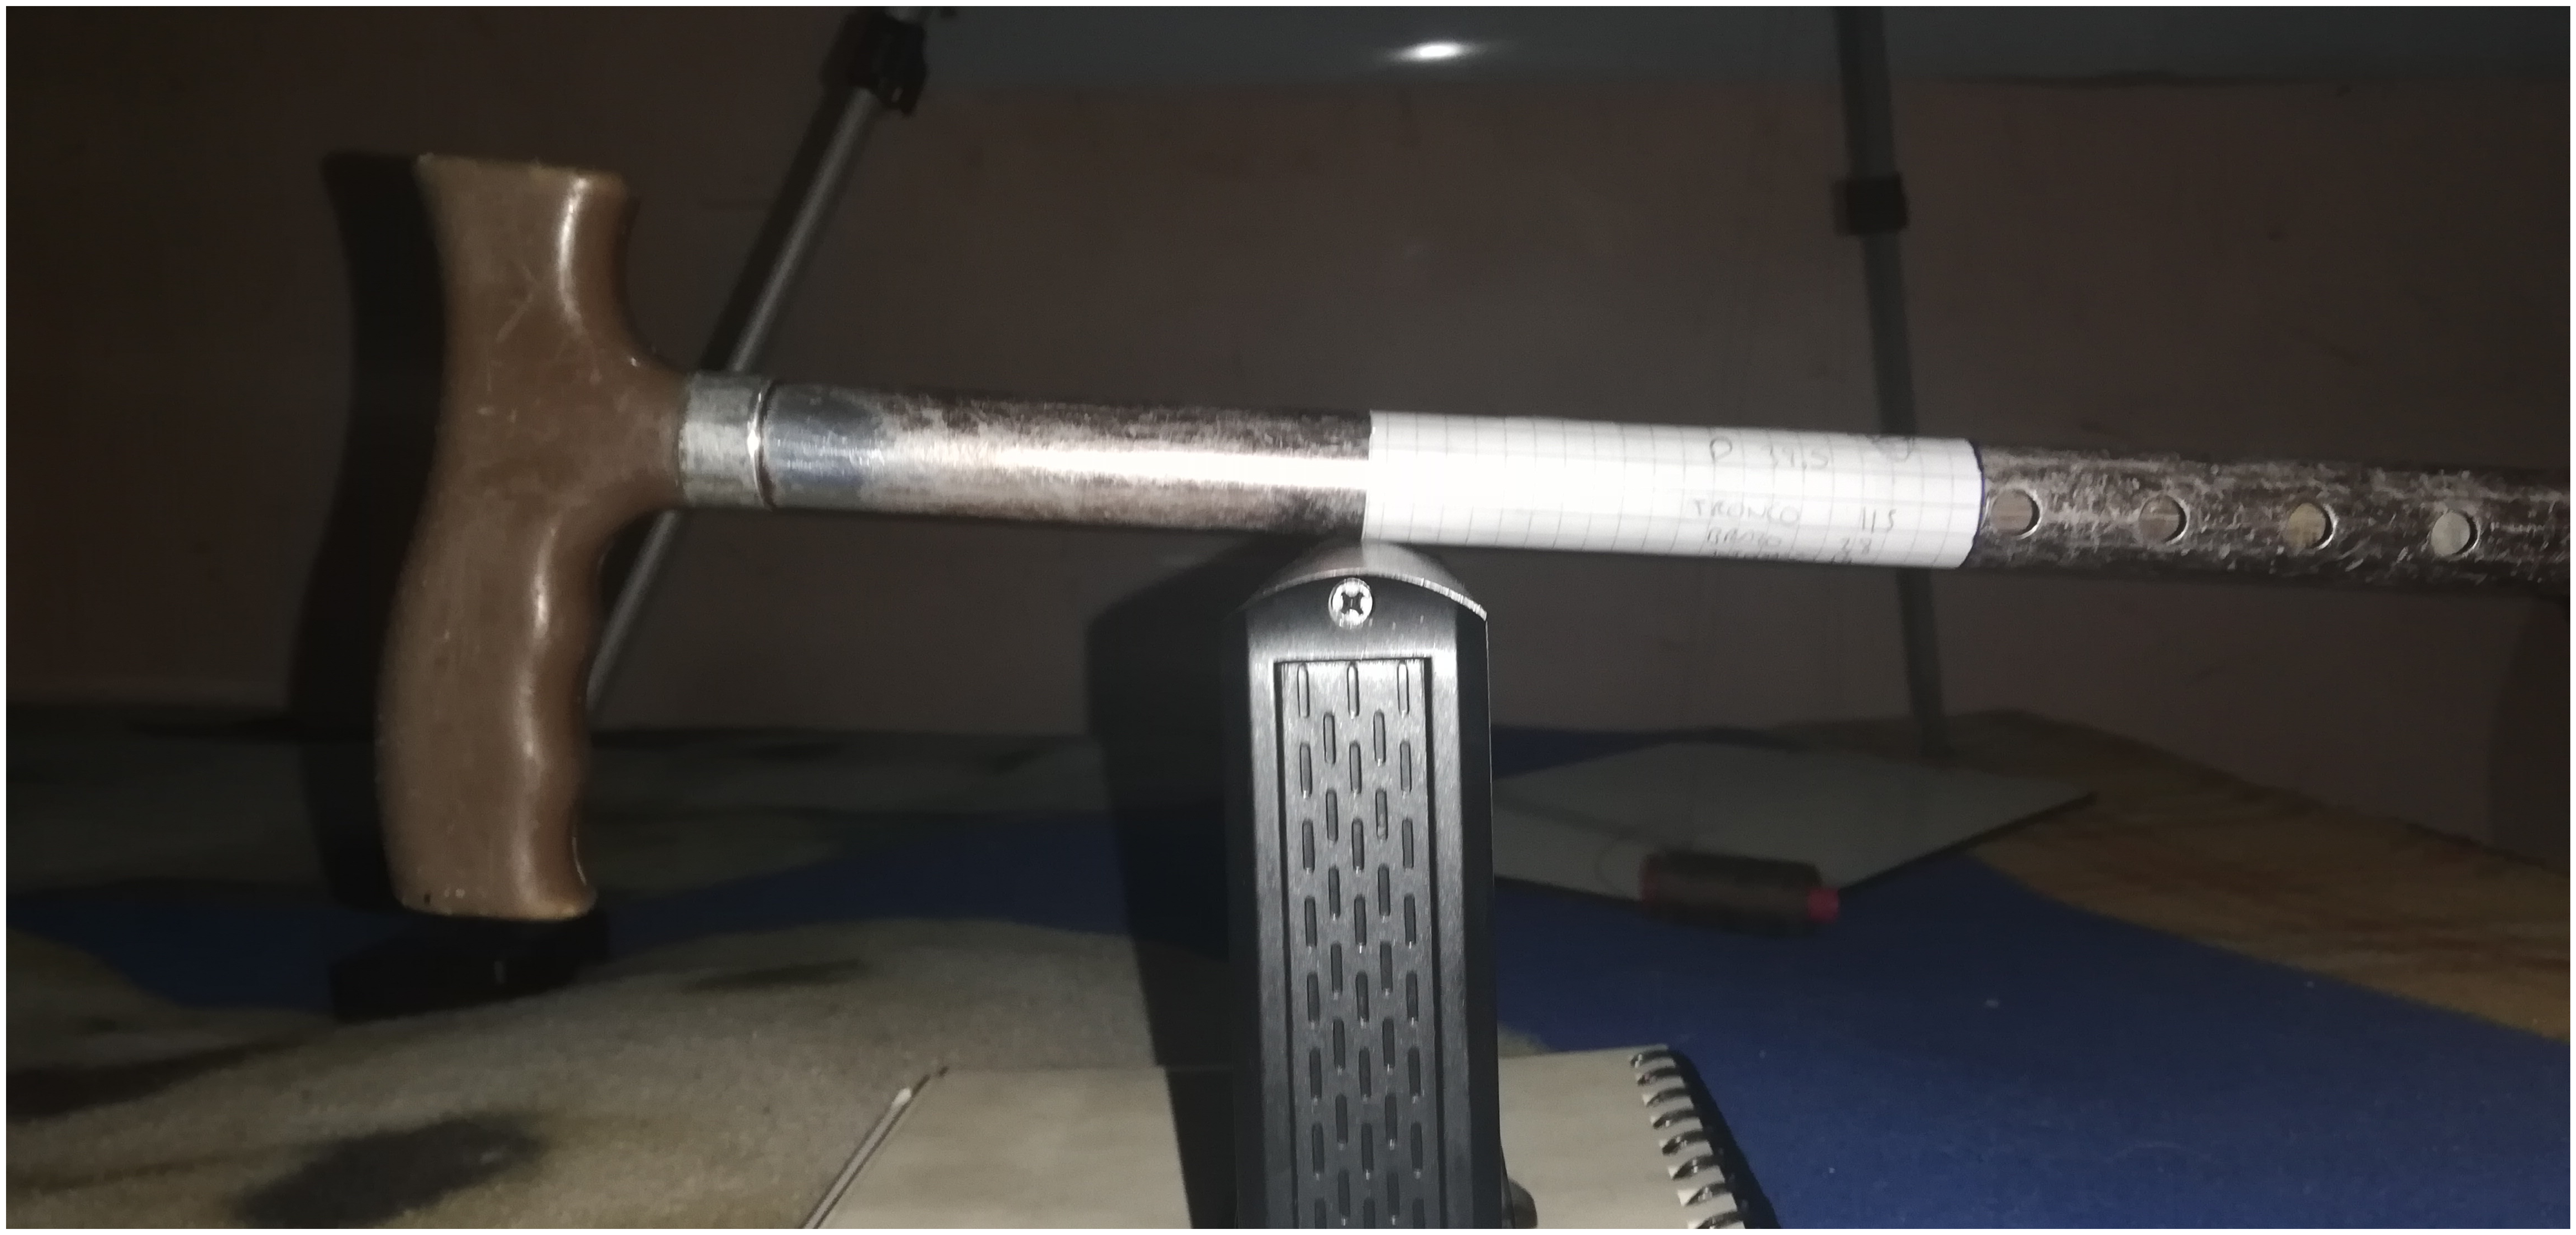
\includegraphics[width=0.65\textwidth]{resources/f4.eps}
\caption{Calculo experimental del centro de masa del bastón.}
\label{figura4}
\source{Fotografía propia.}
\end{figure}

Posteriormente se calculo el centro de masa del bastón con la ayuda de un apoyo
curvilíneo al cual fue suspendido hasta el equilibrio, como se observa en la
\textbf{Figura \ref{figura4}}.

Para la medición se escoge un valor de distancia ($b$), que se mantendrá
constante durante la medición, y se registrarán 2 veces la cantidad de tiempo
que requiere el péndulo para hacer una cantidad determinada de oscilaciones
completas tal que la amortiguación natural causada por la fricción entre el
objeto y el eje no degrade la oscilación.

Una vez medidos los datos para 5 valores distintos de distancia ($b$), se
procederá a calcular el periodo ($T$) con la siguiente ecuación:

\begin{equation}
    T = \frac{\bar{t}}{n}
\label{promedio}
\end{equation}
\vspace{0.10cm}

Donde $\bar{t}$, es el promedio de las mediciones realizadas, y $n$ el numero de
oscilaciones sin amortiguación significativa.

Luego se procederá a graficar la relación distancia ($b$) vs. periodo ($T$),
para realizar primeramente la linealización de la curva por medio de un cambio
de variable, el calculo de la recta por el método de los mínimos cuadrados, y
posteriormente hallar la relación funcional entre las variables.

Finalizando con el calculo del valor del radio de giro y la gravedad, a partir
de las \textbf{Ecuación \ref{funcional}}:

\begin{equation*}
    A = -k^2
\end{equation*}
\begin{equation*}
    B = \frac{g}{4\pi^2}
\end{equation*}
\vspace{0.10cm}

Donde $A$ y $B$ son los parámetros de la recta de ajuste.

Despejando $k$, se obtiene:

\begin{equation}
    k = \sqrt{-A}
\label{radiodegiro2}
\end{equation}
\vspace{0.10cm}

Despejando $g$, se obtiene:

\begin{equation}
    g = 4\pi^2\, B
\label{gravedad}
\end{equation}
\vspace{0.10cm}

\textbf{Datos tomados en el experimento:} \\

En el \textbf{Cuadro \ref{cuadro2}}, se pueden ver los valores tomados del 
experimento, tanto la distancia ($b$), como el tiempo de $n$ oscilaciones
tomados 2 veces, además del valor del periodo resultante.

\begin{table}[!h]
\begin{center}
\begin{tabular}{|c||>{\centering}m{1.5cm}<{\centering}|
                   |>{\centering}m{1.5cm}<{\centering}
                   |>{\centering}m{1.5cm}<{\centering}
                   |>{\centering}m{1.5cm}<{\centering}|
                   |>{\centering}m{1.5cm}<{\centering}|}
\hline
$i$ & $b_i [cm]$ & $n_i$ & $t_{1i} [s]$ & $t_{2i} [s]$ & $T_i [s]$
    \tabularnewline \hline \hline
1 & 33.5 & 10 & 12.73 & 12.78 & 1.2755 \tabularnewline \hline
2 & 31.0 &  8 &  9.85 &  9.99 & 1.2400 \tabularnewline \hline
3 & 28.5 &  6 &  7.23 &  7.31 & 1.2117 \tabularnewline \hline
4 & 26.0 &  5 &  5.88 &  5.95 & 1.1830 \tabularnewline \hline
5 & 23.5 &  4 &  4.59 &  4.66 & 1.1563 \tabularnewline \hline
\end{tabular}
\caption{Mediciones de tiempo en función de la distancia en el péndulo.}
\label{cuadro2}
\source{Elaboración propia.}
\end{center}
\end{table}

\section{Resultados}

\begin{figure}
\centering
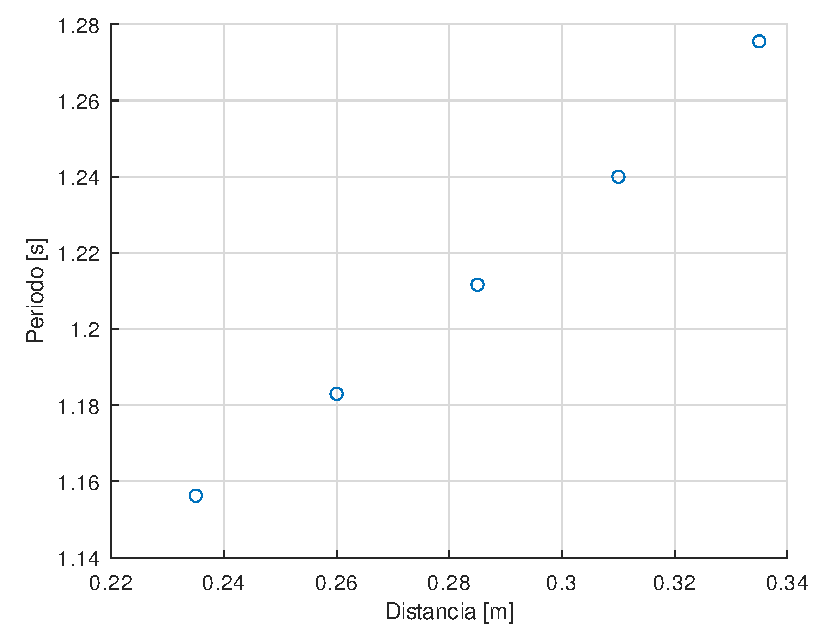
\includegraphics[width=0.75\textwidth]{resources/o1.1.eps}
\caption{Gráfica de distancia vs periodo.}
\label{figura5}
\source{Elaboración propia.}
\end{figure}

A partir de los datos obtenidos se calculó el periodo de oscilación ($T$) para
los valores de distancia ($b$), con los que se generó la gráfica de la
\textbf{Figura \ref{figura5}}.

Posteriormente se linealizó la curva por medio de un cambio de variable, y se
calculó la recta de mejor ajuste por el método de los mínimos cuadrados,
resultando los siguientes valores:

\begin{equation*}
    A = (-0.0225 \pm 0.0008) [m^2]; 3.67\%
\end{equation*}
\begin{equation*}
    B = (0.248 \pm 0.002) [m/s^2]; 0.77\%
\end{equation*}
\vspace{0.10cm}

Siendo su coeficiente de correlación ($r$):

\begin{equation*}
    r = 0.9999
\end{equation*}
\vspace{0.10cm}

Resultando el modelo de ajuste:

\begin{center}
\begin{tabular}{|>{\centering}m{9.2cm}<{\centering}|}
\hline
\textbf{Resultado} 
\tabularnewline \hline
\\
$b^2 = -0.0225 + 0.248\,b\,T^2$ \tabularnewline
\\
\hline
\end{tabular}
\end{center}
\vspace{0.10cm}

Para el calculo del radio de giro ($b$) se utiliza la
\textbf{Ecuación \ref{radiodegiro2}}, resultando:

\begin{center}
\begin{tabular}{|>{\centering}m{9.2cm}<{\centering}|}
\hline
\textbf{Resultado} 
\tabularnewline \hline
\\
$k = (0.1501 \pm \num{1.3992e-6}) [m]; \num{9.3188e-4}\%$ \tabularnewline
\\
\hline
\end{tabular}
\end{center}
\vspace{0.10cm}

Para el calculo de la gravedad ($g$) se utiliza la
\textbf{Ecuación \ref{gravedad}}, resultando:

\begin{center}
\begin{tabular}{|>{\centering}m{9.2cm}<{\centering}|}
\hline
\textbf{Resultado} 
\tabularnewline \hline
\\
$g = (9.78 \pm 0.08) [m/s^2]; 0.77\%$ \tabularnewline
\\
\hline
\end{tabular}
\end{center}
\vspace{0.10cm}

\section{Discusión}

Si bien los datos obtenidos aproximan al valor de la gravedad, se notaron dos
inconvenientes en el experimento:

\begin{enumerate}
\item La amortiguación impide tomar múltiples oscilaciones entre menor sea
la distancia entre el centro de masa y el eje de oscilación. Por lo cual para
cada valor de $b$, se estableció un cantidad óptima de oscilaciones, de forma
que no afectasen la medición del periodo $T$.
\item Al ser números pequeños cualquier variación mínima en el cronometrado
de las oscilaciones puede variar el valor de la gravedad $g$ y el radio de giro
$k$ de forma apreciable.
\end{enumerate}

\section{Conclusiones}

Se verificaron las ecuaciones planteadas en la introducción, así como la
ecuación de un oscilador armónico simple para el caso de un péndulo físico.

También se calculó el valor del radio de giro, y la gravedad, siendo este un
valor bastante aproximado al valor teórico de esta ultima.

\begin{thebibliography}{99}

\bibitem{Young&Freedman} Young, Hugh D. y Freedman, Roger A. (2013).\\
Física Universitaria. Volumen 1.\\
13va Edición.\\
Capitulo 14.

\bibitem{GUIA} Departamento de Física - UMSS.\\
Laboratorio de Física Básica II.\\
Guía - Cartilla de laboratorio.\\
Gestión I/2020.

\bibitem{WIKI1} Péndulo simple \\
Extraído el 27 de Abril del 2021, de: \\
\url{https://es.wikipedia.org/wiki/P%C3%A9ndulo_simple}.

\bibitem{RADIO} Radio de giro \\
Extraído el 12 de Mayo del 2021, de: \\
\url{http://momentosdeinercia.blogspot.com/p/blog-page.html}.

\end{thebibliography}

\newpage
\section*{Apéndice A: Cálculos adicionales}

\subsection{Linealización de la curva}

Conociendo $t_{1i}$, $t_{2i}$, se calculan los valores del promedio ($\bar{t}$),
y el periodo de oscilación ($T$), para el numero de oscilaciones ($n_i$) que se
midieron, en el \textbf{Cuadro \ref{cuadro3}}.

\begin{table}[!h]
\begin{center}
\begin{tabular}{|c||>{\centering}m{2.0cm}<{\centering}
                  |>{\centering}m{2.0cm}<{\centering}
                  |>{\centering}m{2.0cm}<{\centering}|
                  |>{\centering}m{1.2cm}<{\centering}
                  |>{\centering}m{2.0cm}<{\centering}|}
\hline
$i$ & $t_{1i} [s]$ & $t_{2i} [s]$ & $\bar{t}_i [s]$ & $n_i$ & $T_i [s]$
    \tabularnewline \hline \hline
1 & $12.7300$ & $12.7800$ & $12.7550$ & 10 & $1.2755$ \tabularnewline \hline
2 & $ 9.8500$ & $ 9.9900$ & $ 9.9200$ &  8 & $1.2400$ \tabularnewline \hline
3 & $ 7.2300$ & $ 7.3100$ & $ 7.2700$ &  6 & $1.2117$ \tabularnewline \hline
4 & $ 5.8800$ & $ 5.9500$ & $ 5.9150$ &  5 & $1.1830$ \tabularnewline \hline
5 & $ 4.5900$ & $ 4.6600$ & $ 4.6250$ &  4 & $1.1563$ \tabularnewline \hline
\end{tabular}
\caption{Calculo del periodo de oscilación.}
\label{cuadro3}
\source{Elaboración propia.}
\end{center}
\end{table}

En el \textbf{Cuadro \ref{cuadro4}}, se detallan los valores con los cambios de
variable $x = b\,T^2$ y $y = b^2$:

\begin{table}[!h]
\begin{center}
\begin{tabular}{|c||>{\centering}m{2.5cm}<{\centering}
                  |>{\centering}m{2.5cm}<{\centering}|}
\hline
$i$ & $x_i (b\,T^2)$ & $y_i (b^2)$ \tabularnewline \hline \hline
1 & 0.5450 & 0.1122 \tabularnewline \hline
2 & 0.4767 & 0.0961 \tabularnewline \hline
3 & 0.4184 & 0.0812 \tabularnewline \hline
4 & 0.3639 & 0.0676 \tabularnewline \hline
5 & 0.3142 & 0.0552 \tabularnewline \hline
\end{tabular}
\caption{Valores linealizados de $x$ y $y$.}
\label{cuadro4}
\source{Elaboración propia.}
\end{center}
\end{table}

\begin{figure}
\centering
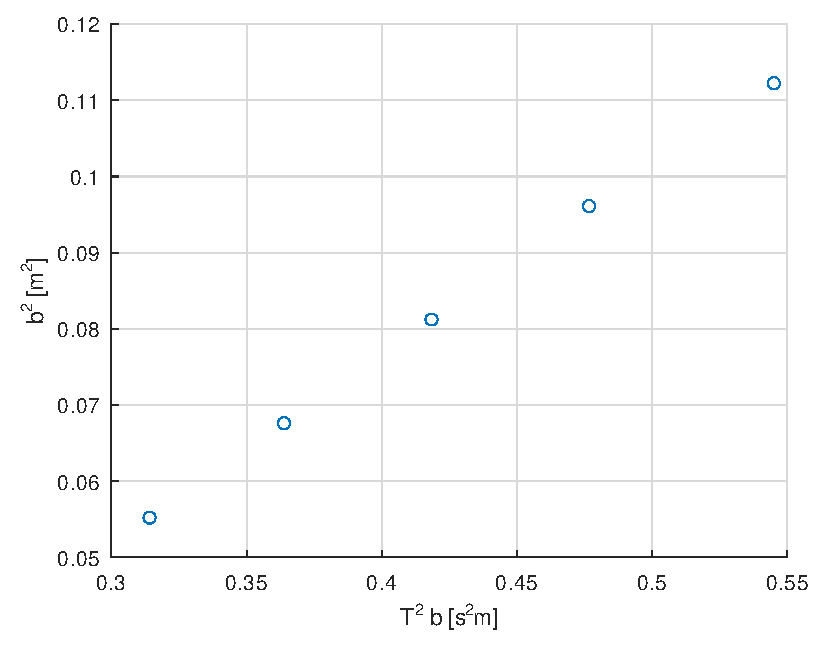
\includegraphics[width=0.75\textwidth]{resources/o1.2.eps}
\caption{Gráfica de $ln(L)$ vs. $ln(T)$.}
\label{figura7}
\source{Elaboración propia.}
\end{figure}

Los valores del \textbf{Cuadro \ref{cuadro4}}, pueden verse gráficamente en la
\textbf{Figura \ref{figura7}}.

\subsection{Método de mínimos cuadrados}

Se calculan los parámetros de la recta por el método de los mínimos cuadrados,
con la ayuda de los datos presentados en el \textbf{Cuadro \ref{cuadro5}}.

\begin{table}[!h]
\begin{center}
\begin{tabular}{|c||>{\centering}m{1.8cm}<{\centering}
                  |>{\centering}m{1.8cm}<{\centering}
                  |>{\centering}m{1.8cm}<{\centering}|
                  |>{\centering}m{1.8cm}<{\centering}
                  |>{\centering}m{1.8cm}<{\centering}
                  |>{\centering}m{2.1cm}<{\centering}|}
\hline
$i$ & $x^2_i$ & $y^2_i$ & $x_i y_i$ &
    $Y_i$ & $d_i\,(\num{e-3}$ & $d^2_i\,(\num{e-6})$
    \tabularnewline \hline \hline
1 & 0.2970 & 0.0126 & 0.0612 & 0.1126 & -0.3422 & 0.1171 \tabularnewline \hline
2 & 0.2272 & 0.0092 & 0.0458 & 0.0956 &  0.4785 & 0.2290 \tabularnewline \hline
3 & 0.1751 & 0.0066 & 0.0340 & 0.0812 &  0.0408 & 0.0017 \tabularnewline \hline
4 & 0.1324 & 0.0046 & 0.0246 & 0.0677 & -0.0605 & 0.0037 \tabularnewline \hline
5 & 0.0987 & 0.0030 & 0.0174 & 0.0553 & -0.1166 & 0.0136 \tabularnewline \hline
\end{tabular}
\caption{Valores para el método de mínimos cuadrados.}
\label{cuadro5}
\source{Elaboración propia.}
\end{center}
\end{table}

\begin{equation*}
    n = 5
\end{equation*}
\begin{equation*}
    \sum x_i = 2.1181
\end{equation*}
\begin{equation*}
    \sum y_i = 0.4124
\end{equation*}
\begin{equation*}
    \sum x^2_i = 0.9304
\end{equation*}
\begin{equation*}
    \sum y^2_i = 0.0360
\end{equation*}
\begin{equation*}
    \sum x_i y_i = 0.1829
\end{equation*}
\begin{equation*}
    \Delta_1 = n \sum x^2_i - \left( \sum x_i \right)^2 = 0.1656
\end{equation*}
\begin{equation*}
    \Delta_2 = n \sum y^2_i - \left( \sum y_i \right)^2 = 0.0102
\end{equation*}
\begin{equation*}
    A = \frac{\sum y_i \sum x^2_i - \sum x_i y_i \sum x_i}{\Delta_1} = -0.0225
\end{equation*}
\begin{equation*}
    B = \frac{n \sum x_i y_i - \sum x_i \sum y_i}{\Delta_1} = 0.2479
\end{equation*}
\begin{equation*}
    \sum d^2 = \num{3.6499e-7}
\end{equation*}
\begin{equation*}
    \sigma^2 = \frac{\sum d^2_i}{n-2} = \num{1.2166e-7}
\end{equation*}
\begin{equation*}
    \sigma_A = \sqrt{\frac{\sigma^2 \sum x^2_i}{\Delta_1}} = \num{8.2672e-4}
\end{equation*}
\begin{equation*}
    \sigma_B = \sqrt{\frac{\sigma^2 n}{\Delta_1}} = 0.0019
\end{equation*}
\vspace{0.10cm}

Parámetros de la recta obtenida:

\begin{equation*}
    A = (-0.0225 \pm \num{8.2672e-4}) [m^2]; 3.6671\%
\end{equation*}
\begin{equation*}
    B = (0.2479 \pm 0.0019) [m/s^2]; 0.7731\%
\end{equation*}
\vspace{0.10cm}

Siendo el coeficiente de correlación:

\begin{equation*}
    R = \frac{n \sum x_i y_i - (\sum x_i)(\sum y_i)}{\sqrt{\Delta_1 \Delta_2}}
      = 0.9999
\end{equation*}
\vspace{0.10cm}

La ecuación de la recta resultante es:

\begin{equation*}
    y = -0.0225 + 0.2479\,x
\end{equation*}
\vspace{0.10cm}

\subsection{Calculo del radio de giro}

Para el calculo del radio de giro, se utiliza la
\textbf{Ecuación \ref{radiodegiro2}}:

\begin{equation*}
    k = \sqrt{-A} = \sqrt{-(-0.0225)} = 0.1501
\end{equation*}
\vspace{0.10cm}

Y el error de la medición es:

\begin{equation*}
    \frac{\partial k}{\partial A} = \frac{1}{2} \sqrt{A^3}
                                  = \frac{1}{2} |A| \sqrt{-A}
\end{equation*}
\begin{equation*}
    e_k = \left(\frac{1}{2} |A| \sqrt{-A}\right) e_A = \num{1.3992e-6}
\end{equation*}
\vspace{0.10cm}

Resultando:

\begin{equation*}
    k = (0.1501 \pm \num{1.3992e-6}) [m]; \num{9.3188e-4}\%
\end{equation*}
\vspace{0.10cm}

\subsection{Calculo de la gravedad}

Para el calculo de la gravedad, se utiliza la \textbf{Ecuación \ref{gravedad}}:

\begin{equation*}
    g = 4 \pi^2\, B = 4\,(3.1415)^2 (0.2479) = 9.7869
\end{equation*}
\vspace{0.10cm}

Y el error de la medición es:

\begin{equation*}
    \frac{\partial g}{\partial B} = 4 \pi^2
\end{equation*}
\begin{equation*}
    e_g = 4 \pi^2\,e_B = 0.0757
\end{equation*}
\vspace{0.10cm}

Resultando:

\begin{equation*}
    g = (9.7869 \pm 0.0757) [m/s^2]; 0.7731\%
\end{equation*}
\vspace{0.10cm}

\newpage
\section*{Apéndice B: Cálculos realizados en \emph{Octave}}

A continuación se presenta los cálculos realizados en el programa \emph{Octave}
para la generación de las gráficas, la linealización de la curva, el calculo
de los mínimos cuadrados, el valor del radio de giro y el valor de la gravedad.

\begin{shaded}
\begin{alltt}
\footnotesize
\# Datos importados (i1.csv):
\input{resources/i1.csv}
\# Comandos ejecutados (o1.m):
\input{../../octave/graficar.m}
\input{../../octave/minimoscuadrados.m}
\input{resources/o1.m}
\# Salida del programa (o1.out):
\input{resources/o1.out}
\normalsize
\end{alltt}
\end{shaded}

\newpage
\section*{Apéndice C: Montaje}

Como comprobación de la autenticidad del trabajo, se adjunta una fotografía del
autor junto con el montaje del experimento, que puede apreciarse en la
\textbf{Figura \ref{figura6}}.

\begin{figure}
\centering
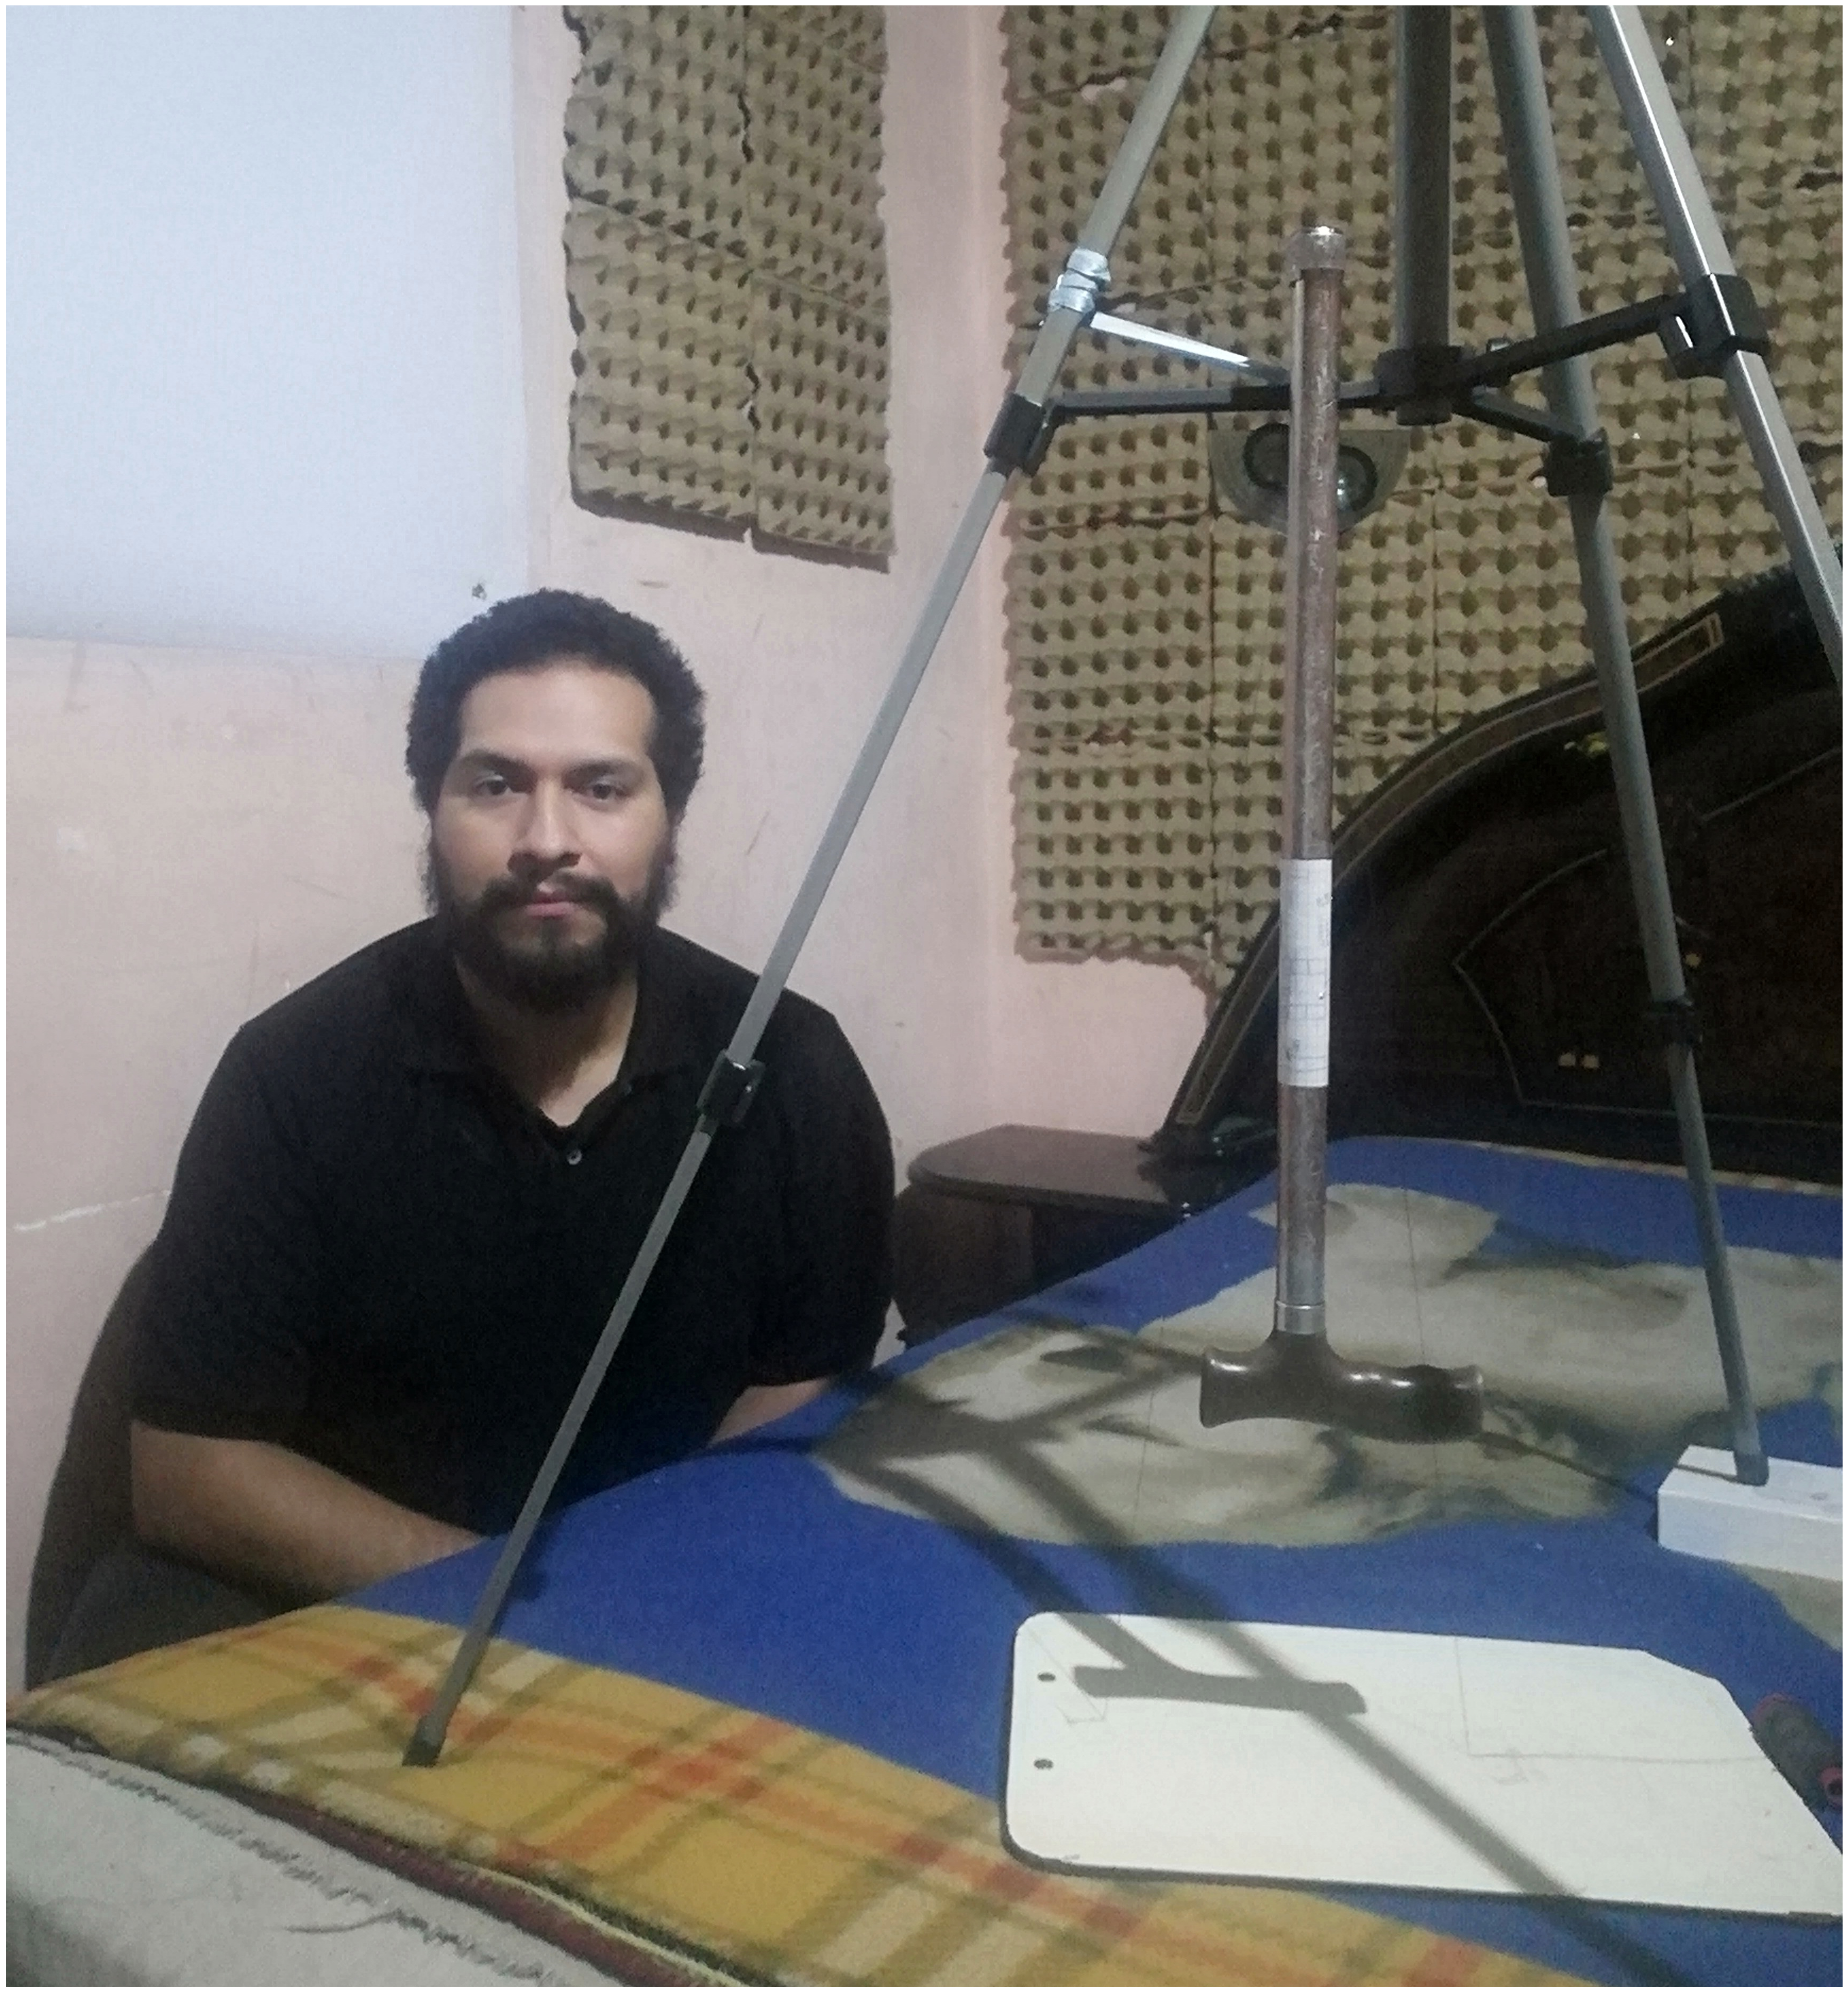
\includegraphics[width=0.75\textwidth]{resources/f5.eps}
\caption{Autorretrato con el montaje del experimento.}
\label{figura6}
\source{Fotografía propia.}
\end{figure}

\end{document}
